\documentclass[sigconf,anonymous]{acmart}

\usepackage[utf8]{inputenc}
\usepackage{listingsutf8}
\usepackage{balance}
\usepackage{booktabs}
\usepackage{multirow}
\usepackage{tabularx}
\usepackage{adjustbox}
\usepackage{makecell}
\usepackage{microtype}
\usepackage{xurl}
\usepackage{seqsplit}
% --- Visual standardization (tables and line breaks) ---
\setlength{\tabcolsep}{4pt}
\renewcommand{\arraystretch}{1.1}
\setlength{\emergencystretch}{2em}
\newcommand{\tcode}[1]{\texttt{\seqsplit{#1}}}

\setcopyright{none}
\settopmatter{printacmref=false}
\renewcommand\footnotetextcopyrightpermission[1]{}
% Conference metadata (CBSoft 2026 / SBLP 2026). Confirm exact dates/venue against the official CFP.
\acmConference[SBLP 2026]{30th Brazilian Symposium on Programming Languages}{September 8--11, 2026}{São Paulo, SP, Brazil}


\title{Gaps in Operator Fusion for Deep Learning Systems: The \textit{Trade-off} Between Compilation and Execution of Unfused Operations}

\newcommand{\best}[1]{\textcolor{blue}{#1}}
\newcommand{\worst}[1]{\textcolor{red}{#1}}

\renewcommand\abstractname{ABSTRACT}
\renewcommand\keywordsname{KEYWORDS}
\renewcommand\refname{REFERENCES}

\author[L. Kamei]{Leonardo Yukio Macedo Kamei}
\affiliation{%
  \institution{PUC-MG}
  \city{Belo Horizonte}
  \country{Brazil}}
\email{leokamei1@gmail.com}

\author[P. Costa]{Pedro Henrique Ramos Costa}
\affiliation{%
  \institution{PUC-MG}
  \city{Belo Horizonte}
  \country{Brazil}}
\email{phramoscosta@gmail.com}

\begin{document}

\begin{abstract}
Operator fusion trades compilation time for execution efficiency, but this cost is often hidden. In modern compilers such as PyTorch~2 (\textit{TorchInductor}) and XLA, heuristics and constraint rules prevent the fusion of common kernels like BatchNorm+ReLU and BatchNorm~$\rightarrow$~Conv, which, if fused, can affect both compilation and execution times. In this paper, we algebraically formalize the trade-off between compilation-time and execution-time gains during Operator Fusion passes in modern machine learning compilers. At the core of our proposal is a framework that models the total cost of a backend as $T(n)=T_C+n\,T_X$, where $T_C$ is the compilation time, $T_X$ the per-execution latency, and $n$ the number of executions, making explicit the regime in which each compiler is preferable. We also show empirically that, with respect to time-to-first-batch, PyTorch~2 performs fusion passes in a suboptimal order, and we propose an alternative optimization sequence. Finally, we provide a real-world benchmark and a tool to indicate the best backend according to the usage regime.
\end{abstract}

\keywords{Operator Fusion, Machine Learning Compilers, Compilation Time, Kernel Fusion, Performance Benchmarking}

\maketitle


\section{Introduction}
The \emph{operator fusion} technique has direct roots in classical compiler optimizations, such as \emph{loop} fusion, historically used to increase parallelism and improve data locality \cite{wolf1991wolf}. In modern compilers for Machine Learning, particularly on GPUs, this technique plays a central role: by combining multiple operations into a single \emph{kernel}, memory traffic is reduced, intermediate tensors are avoided, and the number of dynamic launches during execution is decreased \cite{chen2018tvm,liu2021dnnfusion}. Systems such as XLA, TVM, TensorRT, and the TorchInductor backend adopt aggressive fusion to amortize CPU--GPU communication costs and consolidate operator sequences into larger, more efficient \emph{kernels} \cite{xla2017leary,chen2018tvm,pytorch2022}.

Fusion is performed over the program's control-flow graph (CFG). However, deciding \emph{what} and \emph{how} to fuse in modern graphs is challenging: optimal fusion plans are, in general, NP-hard problems \cite{darte1999,10.5555/645671.665526}. For this reason, compilers adopt heuristics that seek to balance \textbf{compilation time} and \textbf{execution time}. This balance is especially important in dynamic workloads (with variable \emph{shapes}) and in scenarios with few repetitions, where the cost up to the first execution dominates the perceived performance.

Despite this impact, the literature usually favors latency metrics and ignores compilation time. There is no standard protocol for making explicit when it pays off to compile more aggressively in exchange for faster execution, leaving practitioners without a principled way to choose among backends. XLA \cite{snider2023xla}, TVM \cite{chen2018tvm}, and TorchInductor (PyTorch~2) \cite{pytorch2022} each take a different approach---rule-based fusion, cost-model-guided exploration, and local code generation, respectively---resulting in very different compilation- and execution-time profiles across usage regimes.

We evaluate the \emph{trade-off} between these two times across the TVM, XLA, and TorchInductor compilers under a common protocol. The core of our proposal is a framework that, for a number of executions \(n\), models the total cost of each \emph{backend} as \(T_b(n)=a_b n + b_b = T_C + n\,T_X\), where \(b_b = T_C\) is the compilation time and \(a_b = T_X\) is the per-execution latency (Section~\ref{sec:methodology}); minimizing \(T_b(n)\) over the backends identifies which one is preferable in each usage regime. We also investigate the fusion heuristics used by the compilers and propose a new execution order that simultaneously reduces compilation time and execution time on real-world models.

\textbf{Contributions:}
\begin{itemize}
    \item An algebraic framework, \(T(n)=T_C+n\,T_X\), formalizing the trade-off between compilation time (\(T_C\)) and execution time (\(T_X\)) of ML (\textit{Machine Learning}) models with respect to \textit{kernel} fusion heuristics;
    \item Analysis and benchmarking of the XLA, PyTorch, and TVM models in terms of our algebraic framework;
    \item Artifact analysis (TVMScript, HLO, Triton) to quantify and analyze fusion granularity per \emph{backend}, mapping patterns by architecture (ResNet-18/50, BERT, and GPT-2) and their impact on latency;
    % \item A proposal of a new optimization order for PyTorch during Fusion.
\end{itemize}

\section{Theoretical Background}
\label{sec:background}

Consider a sequence of operators $x_{k+1}=f_k(x_k)$ and $x_{k+2}=f_{k+1}(x_{k+1})$, in which each $f_i$ acts on tensors of a computation graph. We say that $f_k$ and $f_{k+1}$ are \emph{fusible} when there exists a single operator $h$ such that $h(x_k)=f_{k+1}(f_k(x_k))$ and the execution of $h$ preserves every observable semantics of the original sequence. In this case, the compiler performs the transformation $(f_k,f_{k+1})\Rightarrow h$, eliminating the materialization of intermediate tensors, reducing the number of kernel launches, and improving memory locality.

This notion of fusibility is the computation-graph analogue of classical \emph{peephole optimization}, as we detail in Section~\ref{sec:related}: $h$ plays, for a window of graph operators, the role that an equivalent instruction plays for a window of three-address-code instructions. In ML models, however, operators handle multi-dimensional tensors and their definitions are often complex. We therefore focus on three fusions, defined by Equations~(III), (VIII), and~(XIV) in Appendix~\ref{app:fusions}: \tcode{BatchNorm+ReLU}, \tcode{Conv+BatchNorm+ReLU}, and the affine part of \tcode{LayerNorm} folded into \tcode{Linear}.

Some kernel sequences are intentionally left unfused, owing to conservative rules that prevent incorrect execution or unpredictable performance:
\begin{itemize}
    \item \textbf{Training mode.} In training, \tcode{BatchNorm} depends on the statistics of the current batch and on the update of internal state. Fusing it may break correctness, since it prevents the reuse of intermediate values needed for the gradient.
    \item \textbf{Canonical form.} Fusion requires the operators to be in direct sequence in the CFG, with no intervening operations and no multiple consumers, which preserves the original semantics.
    \item \textbf{Numerical precision.} Precision mismatches (e.g., \tcode{BatchNorm} in FP32 and \tcode{ReLU} in FP16) can make fusion unsafe due to overflow or underflow risks.
    \item \textbf{Shape compatibility.} Fusion candidates must have compatible shapes; mismatches may require reindexing or broadcasting, making fusion infeasible.
    \item \textbf{Operation type.} Not every operation is fusible: differing memory-access patterns or synchronization requirements may prevent execution in a single kernel.
    \item \textbf{Backend restrictions.} Calls to external libraries (e.g., cuDNN or cuBLAS) and non-deterministic operations limit fusibility, since the compiler does not control their internal execution.
\end{itemize}
In every case, the fusion decision involves an explicit trade-off: investing more compilation time to reduce execution time, or compiling quickly with fewer fusions. This balance underlies the cost model adopted in this work and guides the comparison between backends.

\section{Methodology}
\label{sec:methodology}

We compare \textit{TVM} \cite{chen2018tvm}, \textit{XLA} \cite{snider2023xla}, and \textit{TorchInductor} (PyTorch~2) \cite{pytorch2022} in a controlled environment, measuring \textbf{compilation time}, \textbf{average latency per execution}, and \textbf{fusion granularity}.

\subsection{Experimental Environment}

All experiments were run on the same computing system. The base environment consists of a Fedora~41 operating system, using kernel~6.16.12, with an AMD Ryzen~5~4600G CPU and 15.4~GiB of RAM. The GPU was an NVIDIA RTX~3050 with 8~GB of VRAM, operating with driver version~580.95.05. The CUDA stack comprised the CUDA~13.0 driver and the \textit{nvcc} compiler version~12.6 (V12.6.77).

\paragraph{Per-framework configuration.}
For the \textbf{TVM} experiments, we used Python~3.11.13, cuDNN version~9.1 (via PyTorch), TVM~0.22.dev0 (commit~3b60f1c), LLVM~20.1.8, and CUDA~12.6 integrated into the TVM backend.

For \textbf{XLA/TorchInductor}, the experiments were conducted with Python~3.10.18. The XLA backend used JAX/jaxlib~0.6.2, with PJRT (\tcode{jax-cuda12-pjrt}~0.6.2) and cuDNN~9.10.2.21 installed via \textit{pip}. For TorchInductor, we used PyTorch~2.5.1+cu121, executing on device \tcode{cuda:0}.

We used the same hardware/OS and software \emph{stack} per \emph{backend}. Standardized conditions: \tcode{TF32} enabled, \textit{channels\_last} layout, \tcode{cudnn.benchmark=True}, all models in \tcode{eval()}, \emph{warmup}, and explicit separation between compilation and execution. We used an isolated environment for \textbf{TVM} version \tcode{0.22.dev0}.

\subsection{Models and Inputs}
We evaluated \textbf{ResNet-18/50}, \textbf{BERT}, and \textbf{GPT-2}. Inputs for ResNets (CNNs): \tcode{(1,3,224,224)}, \tcode{(16,3,224,224)}, \tcode{(64,3,224,224)}, \tcode{(1,3,512,512)}, \tcode{(1,3,1024,1024)}. Inputs for Transformers: \tcode{(batch, seq\_len)} pairs in \tcode{(1,64)}, \tcode{(1,128)}, \tcode{(8,128)}.

The \textbf{ResNet-18/50}, \textbf{BERT}, and \textbf{GPT-2} models were chosen because they represent distinct and complementary architectural patterns. The ResNets characterize classical convolutional architectures, with recurring \textit{Conv--BatchNorm--ReLU} chains, which are canonical cases for analyzing operator fusion in CNNs.

BERT represents \textit{Transformer} architectures based on encoders, dominated by matrix multiplications, linear projections, normalizations, and activations, allowing us to evaluate fusion strategies on attention-centric graphs.

GPT-2, in turn, exemplifies autoregressive \textit{decoder-only} models, with a more linear and repetitive computational flow, typical of generative models, in which fusion granularity directly affects inference latency.

Together, these models allow us to analyze the behavior of fusion heuristics across different computational and architectural regimes.

\subsection{Experimental Pipeline}
\label{sec:pipeline}
The benchmark workflow adopts four sequential stages, standardized across all models and backends (TVM, XLA, and TorchInductor):

\paragraph{(1) Compilation.}
For each \textit{(model, input)} pair, the compilation time (\tcode{compile\_ms}) is recorded in an isolated process with fixed driver and library versions, focusing primarily on the cost of code generation.

\paragraph{(2) Warmup and execution + graph capture.}
Execution occurs in two phases: (i) a \textit{warmup} phase, focused on building caches and performing \textit{autotuning}; and (ii) a phase of \textit{valid}, timed \textit{executions}. During (ii), the benchmark exports the CFGs of the intermediate representations (IRs) of the analyzed backends [HLO (XLA), TVMScript and TIR (TVM), IR and Triton (TorchInductor)]. We also collect \textit{kernel} metadata when available.

\paragraph{(3) Analysis of kernel quantity and quality.}
From the captured IRs, we perform a structural analysis of the \textit{kernels} generated by each backend. This stage includes quantifying the total number of \textit{kernels}, distinguishing between internal \textit{kernels} and external library calls, as well as qualitatively characterizing the fusions performed. This analysis allows us to evaluate fusion granularity and the degree of delegation to optimized libraries, providing structural context for interpreting the performance results.

\paragraph{(4) Measurements and algebraic model.}
The metrics collected include: \textit{time to first batch} (\tcode{ttfb\_ms}), \textit{average latency per execution} $a$, and \textit{standard deviation} over the 50 valid executions (\tcode{exec\_ms\_mean}, \tcode{exec\_ms\_std}). For \textbf{XLA/TVM}, the compilation time is \textbf{explicitly} separated from the first compiled call $b$. For \textbf{TorchInductor}, the compilation time is estimated by
\[
\mathrm{compile\_time}=\mathrm{first\_call\_ms}-\mathrm{time\_per\_run\_ms},
\]
where \textit{first\_call\_ms} aggregates compilation+execution and \textit{time\_per\_run\_ms} is the average of the subsequent executions.

\textbf{\textit{Algebraic model.}}
We propose an algebraic model for computing the cost of compilation and batched execution across the three analyzed backends, given by:
\[
T_b(n) = a_b\,n + b_b,
\]
where $b_b$ is the fixed cost of compilation and initial overhead, and $a_b$ is the average latency, allowing us to infer the inflection point for different backends as a function of the number of repetitions $n$. Equivalently, writing $b_b = T_C$ (compilation time) and $a_b = T_X$ (per-execution latency), the model reads $T_b(n) = T_C + n\,T_X$; this is the framework we use throughout to compare backends.

The model \(T_b(n) = a_b n + b_b\), together with its \emph{lower envelope}---the curve that, for each value of \(n\), selects the smallest cost among all backends---helps explain the crossover points observed between the different \emph{backends}. Thus, the intersections of these functions indicate from which input size \(n\) each backend becomes more advantageous.

\paragraph{(5) Applying \textit{fold} and comparing regimes.}
In addition to the standard models, we evaluated an alternative scenario in which a \textit{fold} transformation is applied \textbf{before} the regular operator fusion. The \textit{fold} consists of an algebraic reparameterization that absorbs linear operations (such as \textit{BatchNorm} or the affine part of \textit{LayerNorm}) into the parameters of the subsequent operator, explicitly removing these operations from the graph in inference mode.

Unlike operator fusion, which combines multiple operations into a single \textit{kernel} during \textit{codegen}, the \textit{fold} structurally simplifies the graph before code generation. As a consequence, the \textit{fold} mainly affects the fixed compilation cost, reducing \textit{codegen} complexity, while its effects on per-execution latency tend to be smaller or non-deterministic.

For operations with fold, we assume $T_f(n) = a_f \, n + b_f$ to be the cost in backends that perform the \textit{fold} operation before regular operator fusion. Thus, the equivalence point in the number of \textit{batches} $n$ for which $\Delta T = T_f(n) - T_b(n) = 0$, where $T_b(n)$ is the cost in the compiled backend without the fold operation, is given by:
\begin{align*}
n_{\text{eq}}
  = \mathrm{MAX}\!\left(0,\ \frac{b_b - b_f}{a_f - a_b}\right),
   \qquad \text{provided } \Delta a \neq 0.
\end{align*}

\paragraph{(6) \texttt{JSON} construction.}
For each \textit{(model, input, backend)}, including the models with \tcode{fold}, we generate a \tcode{JSON} that consolidates the benchmark state. It includes the experiment identification, time metrics, fused \textit{kernels}, and other metadata.

\subsection{Execution per Compiler and Model}
For each (\textbf{compiler}, \textbf{model}) pair, we run the pipeline [Section~\ref{sec:pipeline}]: (i) graph compilation, (ii) input preparation, (iii) execution of the chosen protocol (10 \emph{warmups} and $n = 50$), (iv) computation of mean, standard deviation, and CI (95\%), and (v) export of metrics and artifacts.

\subsection{Artifact Analysis Script (TVMScript, HLO, Triton)}
We implemented a \textbf{Python script} that performs textual \emph{parsing} of the program tree and produces an artifact.

\subsection*{Reproducibility and Code Availability}
The source code, measurement scripts, and artifacts (HLO/TVMScript/Triton) are available at:
\url{https://github.com/kameczera/compilers-benchmark}

\section{Evaluation}
\label{sec_eval}

The metrics collected include: (i) the number of \emph{kernel} launches at the start and end of the pipeline; (ii) the number of internal and external \emph{kernels}; and (iii) specific decompositions (Triton \emph{kernels}, for example). For \textbf{TVM} we followed the pipeline indicated in the documentation. For \textbf{TorchInductor}, we followed direct execution via PyTorch. For \textbf{XLA}, we report the number of fusions and custom calls.

The PyTorch and XLA models were loaded from native libraries. For TVM, an export step from the PyTorch models was required. This step affects the TVM metrics, since the export process tends to fragment \textit{kernels}. Some operations that are treated as atomic in PyTorch (or encapsulated in optimized library calls) are decomposed by TVM into multiple simpler operators in its IR, which increases the number of generated \textit{kernels} and reduces subsequent fusion opportunities.

% --- Figure 1: Fusion rate ---
\begin{figure}[h]
    \includegraphics[width=0.9\linewidth]{images/comparison.png}
    \caption{Fusion rate per model, considering only internal \emph{kernels}.}
    \label{fig:fusion_rate}
\end{figure}

In Figure~\ref{fig:fusion_rate} we see the rate of fused kernels across the three backends for the four models. Although both \textbf{TorchInductor} and \textbf{XLA} are able to fuse more \textit{kernels} than \textbf{TVM}, the fusion rate of \textbf{XLA} is higher across all models except BERT (Figure~\ref{fig:fusion_rate}). The dominance of \textbf{TorchInductor} and \textbf{XLA} is clearer in Figure~\ref{fig:kernels_interno}. There, we notice a greater weight of external dependencies (external \textit{kernels}), which also affects operator fusion time. In Figure~\ref{fig:kernels_interno} we also observe the number of internal \textit{kernels} per backend in each model.

We caution that these fusion rates are only partially comparable across backends, because the three compilers do not ingest the same intermediate representation of a given model. As noted above, the PyTorch$\rightarrow$TVM export fragments operators that PyTorch treats as atomic, inflating TVM's kernel count and lowering its apparent fusion rate. A strictly isonomic comparison would require feeding all backends the same operator-level representation and applying identical pattern-rewriting rules, so that the same fusion effects could be triggered everywhere; we therefore read these rates as backend-internal indicators rather than as a head-to-head ranking, and leave such a normalized comparison as future work.

\begin{figure}[h]
    \includegraphics[width=0.8\linewidth]{images/external_kernels.png}
    \caption{Number of external \textit{kernels}.}
    \label{fig:kernels_externo}
\end{figure}

\begin{figure}[h]
    \includegraphics[width=0.8\linewidth]{images/internal_kernels.png}
    \caption{Number of internal \textit{kernels}.}
    \label{fig:kernels_interno}
\end{figure}

\subsection{Residual Networks}

\begin{table}[t]
\centering
\caption{ResNet-18 and ResNet-50 --- \textbf{compilation} (ms) and \textbf{execution} time (mean $\pm$ sd, ms; $n=50$, 10 warmups). Best per metric in \best{blue}. 95\% CIs are derivable from sd and $n$.}
\label{tab:resnet_compile_exec}
\footnotesize
\renewcommand{\arraystretch}{1.0}
\adjustbox{max width=\textwidth}{%
\begin{tabular}{ll cc cc}
\toprule
& & \multicolumn{2}{c}{\textbf{ResNet-18}} & \multicolumn{2}{c}{\textbf{ResNet-50}} \\
\cmidrule(lr){3-4}\cmidrule(lr){5-6}
\textbf{Framework} & \textbf{Input (N,C,H,W)} & \textbf{Comp.} & \textbf{Exec.} & \textbf{Comp.} & \textbf{Exec.} \\
\midrule
\multirow{5}{*}{TorchInductor}
& (1,\,3,\,224,\,224)   & \worst{8550} & \best{1.76 $\pm$ 0.03}  & \worst{13902} & \best{3.55 $\pm$ 0.04} \\
& (16,\,3,\,224,\,224)  & \worst{6233} & \worst{11.78 $\pm$ 0.18} & \worst{13125} & \best{29.20 $\pm$ 0.35} \\
& (64,\,3,\,224,\,224)  & \worst{6348} & \worst{40.51 $\pm$ 0.42} & \worst{11952} & \worst{107.14 $\pm$ 1.29} \\
& (1,\,3,\,512,\,512)   & \worst{6168} & \worst{4.70 $\pm$ 0.05}  & \worst{12373} & \worst{10.73 $\pm$ 0.13} \\
& (1,\,3,\,1024,\,1024) & \worst{5929} & \worst{15.07 $\pm$ 0.16} & \worst{11767} & \worst{37.16 $\pm$ 0.45} \\
\midrule
\multirow{5}{*}{TVM}
& (1,\,3,\,224,\,224)   & \worst{10273} & \worst{6.94 $\pm$ 0.07}   & \worst{10273} & \worst{19.47 $\pm$ 0.18} \\
& (16,\,3,\,224,\,224)  & \worst{10004} & \worst{82.53 $\pm$ 0.62}  & \worst{10004} & \worst{247.63 $\pm$ 2.23} \\
& (64,\,3,\,224,\,224)  & \worst{9899}  & \worst{321.09 $\pm$ 1.90} & \worst{9896}  & \worst{986.00 $\pm$ 8.87} \\
& (1,\,3,\,512,\,512)   & \worst{4992}  & \worst{27.00 $\pm$ 0.31}  & \worst{9648}  & \worst{91.01 $\pm$ 0.82} \\
& (1,\,3,\,1024,\,1024) & \worst{9256}  & \worst{103.97 $\pm$ 0.84} & \worst{9256}  & \worst{347.04 $\pm$ 3.12} \\
\midrule
\multirow{5}{*}{XLA}
& (1,\,3,\,224,\,224)   & \best{2457} & \worst{1.99 $\pm$ 0.03}  & \best{4748} & \worst{4.21 $\pm$ 0.04} \\
& (16,\,3,\,224,\,224)  & \best{2917} & \best{11.39 $\pm$ 0.15}  & \best{5936} & \worst{29.71 $\pm$ 0.30} \\
& (64,\,3,\,224,\,224)  & \best{4640} & \best{38.79 $\pm$ 0.39}  & \best{9581} & \best{101.00 $\pm$ 1.01} \\
& (1,\,3,\,512,\,512)   & \best{3050} & \best{4.17 $\pm$ 0.05}   & \best{4671} & \best{10.70 $\pm$ 0.11} \\
& (1,\,3,\,1024,\,1024) & \best{3297} & \best{12.75 $\pm$ 0.12}  & \best{6028} & \best{33.77 $\pm$ 0.34} \\
\bottomrule
\end{tabular}
}
\end{table}

In the \textbf{ResNet-18} and \textbf{ResNet-50} architectures, the three backends reveal structural differences in how each system handles fusions, granularity, and delegation of operations to external libraries.

\textbf{TVM} exhibits the largest number of \emph{kernels} due to its form of representation: the \textit{convolution} and \textit{batch normalization} operations arrive marked as \emph{opaque}, and the compiler has no visibility to apply aggressive fusions. Even the \textit{ReLU} remains isolated. The result is a fragmented pipeline, with simple fusions and little structural reduction of the graph.

\textbf{TorchInductor} relies heavily on \textbf{cuDNN} for convolutions, which prevents it from fusing convolution, \textit{BatchNorm}, and activation into a single \textit{kernel}. However, it performs \textit{BatchNorm+ReLU} fusions within Triton \emph{kernels}. There are fewer launches and the graphs are more compact than TVM's. Nevertheless, the use of Triton for elementwise operations and reductions increases code-generation time, \textbf{which grows proportionally with the model} (Table~\ref{tab:resnet_compile_exec}).

This reduces the total number of launches and, in general, results in more compact graphs than TVM's. However, this hybrid approach carries a cost: using Triton for numerous \textit{elementwise} operations and reductions increases \textit{codegen} time and causes compilation time to grow proportionally with model size, especially noticeable when moving from ResNet-18 to ResNet-50.

For XLA, based on the analysis of the HLOs, we observe that the compiler performs aggressive fusions, combining \emph{convolution + bias + batch norm + activation} into a single cuDNN call. This fusion reduces the number of final \emph{kernels} and results in more cohesive pipelines. Experimentally, this behavior showed a direct impact on reducing compilation time compared to the other backends.

\subsection{Attention-Based Architectures (BERT)}

\begin{table}[t]
\centering
\caption{BERT --- \textbf{compilation} (ms) and \textbf{execution} time (mean $\pm$ sd, ms) per input (\textit{batch, seq\_len}); $n=50$, 10 warmups. Best per metric in \best{blue}.}
\label{tab:bert_compile_exec}
\footnotesize
\renewcommand{\arraystretch}{1.0}
\adjustbox{max width=\linewidth}{%
\begin{tabular}{llcc}
\toprule
\textbf{Framework} & \textbf{Input} & \textbf{Comp.} & \textbf{Exec.} \\
\midrule
\multirow{3}{*}{TorchInductor}
& (1,\,64)   & \worst{13449} & \best{3.49 $\pm$ 0.63} \\
& (1,\,128)  & \worst{12071} & 5.11 $\pm$ 0.73 \\
& (8,\,128)  & \worst{11396} & \worst{31.51 $\pm$ 0.95} \\
\midrule
\multirow{3}{*}{TVM}
& (1,\,64)   & \best{2492}  & \worst{6.78 $\pm$ 0.34} \\
& (1,\,128)  & \best{1564}  & \worst{9.85 $\pm$ 0.49} \\
& (8,\,128)  & \best{1464}  & \worst{63.00 $\pm$ 1.26} \\
\midrule
\multirow{3}{*}{XLA}
& (1,\,64)   & \worst{5474}  & \worst{3.88 $\pm$ 0.26} \\
& (1,\,128)  & \worst{5074}  & 5.27 $\pm$ 0.25 \\
& (8,\,128)  & \worst{5317}  & \best{29.95 $\pm$ 0.32} \\
\bottomrule
\end{tabular}
}
\end{table}

The \textbf{BERT} model has a distinct fusion pattern that reflects its architecture centered on \textit{matmuls}~\cite{pati2021demystifying}, QKV projections, and normalization and activation operations.

\textbf{TVM} tends to produce smaller and more numerous \emph{kernels}. This leads to graph fragmentation, similar to what was seen in the ResNets, but in BERT its fusion rate is higher thanks to the structure, which has long elementary chains that are easily collapsible.

\textbf{TorchInductor} explores fusions aimed at minimizing memory access. It delegates the \textit{matmuls} to external libraries (for example, cuBLAS) \cite{pytorch2022} and focuses on the Triton \emph{kernels}. From the direct analysis of the artifacts and kernels generated by TorchInductor, we observed that the compiler synthesizes structures that correspond, in practice, to typical \emph{Transformer} blocks. These kernel templates are reused throughout the network, which leads to a reduction in the number of launches, although at the cost of higher compilation time.

\textbf{XLA} ends up with more \emph{kernels} than TorchInductor, but practically all of them are \textbf{HLO fusions}: from \textit{GEMM} fusions (\tcode{gemm\_fusion\_dot}, with concatenated QKV weights and embedded epilogues) to fusions dedicated to attention \tcode{softmax} (\tcode{triton\_softmax\_computation}), and large \tcode{kLoop}/\tcode{kInput} fusions that implement full \tcode{LayerNorm} and \tcode{GELU}. These \textit{GEMM} fusions correspond to \textbf{the same 72 matrix multiplications observed in TorchInductor}; however, being highly specialized internal fusions, they already incorporate \textit{bias} operations, QKV concatenation, and \textit{layout} adjustments within a single \emph{kernel}. When the \emph{batch} increases, the cost of these \textit{GEMMs} \textbf{comes to dominate the total execution time}, which renders the overhead due to the larger number of \textit{kernels} irrelevant. This behavior is especially visible in the \((8, 128)\) scenario (Table~\ref{tab:bert_compile_exec}). We stress that we only claim one backend to be faster than another when their 95\% confidence intervals do not overlap. At \((1,128)\), for instance, TorchInductor (\(5.11\pm0.73\)~ms) and XLA (\(5.27\pm0.25\)~ms) have overlapping intervals and are therefore statistically indistinguishable, so we refrain from ranking them at that input; the meaningful gaps appear at larger batches such as \((8,128)\), where the GEMM cost dominates and the intervals separate.

In short, the BERT model highlights how architectural differences affect each compiler's strategy.

\subsection{Autoregressive Attention-Based Models (GPT-2)}

\begin{table}[t]
\centering
\caption{GPT-2 --- \textbf{compilation} (ms) and \textbf{execution} time (mean $\pm$ sd, ms) per input (\textit{batch, seq\_len}); $n=50$, 10 warmups. Best per metric in \best{blue}.}
\label{tab:gpt2_compile_exec}
\footnotesize
\renewcommand{\arraystretch}{1.0}
\adjustbox{max width=\linewidth}{%
\begin{tabular}{llcc}
\toprule
\textbf{Framework} & \textbf{Input} & \textbf{Comp.} & \textbf{Exec.} \\
\midrule
\multirow{4}{*}{TorchInductor}
& (1,\,16)   & \worst{15003} & \worst{3.09 $\pm$ 0.33} \\
& (1,\,128)  & \worst{13327} & \worst{6.12 $\pm$ 0.60} \\
& (8,\,128)  & \worst{19121} & \best{30.40 $\pm$ 0.75} \\
& (8,\,256)  & \worst{18353} & \worst{58.56 $\pm$ 0.74} \\
\midrule
\multirow{4}{*}{TVM}
& (1,\,16)   & \worst{8253}  & \worst{7.80 $\pm$ 0.39} \\
& (1,\,128)  & \worst{10312} & \worst{10.55 $\pm$ 0.53} \\
& (8,\,128)  & \worst{9776}  & \worst{41.21 $\pm$ 1.24} \\
& (8,\,256)  & \worst{9549}  & \worst{79.11 $\pm$ 1.98} \\
\midrule
\multirow{4}{*}{XLA}
& (1,\,16)   & \best{2797}  & \best{2.81 $\pm$ 0.17} \\
& (1,\,128)  & \best{3892}  & \best{5.11 $\pm$ 0.28} \\
& (8,\,128)  & \best{5784}  & \worst{30.84 $\pm$ 0.72} \\
& (8,\,256)  & \best{5562}  & \best{58.38 $\pm$ 0.54} \\
\bottomrule
\end{tabular}
}
\end{table}

The GPT-2 blocks follow a relatively linear decoder-only pattern---autoregressive attention and MLP, each preceded by LayerNorm and followed by GELU activation, repeated across all layers \cite{radford2019language}.

\textbf{TVM} cannot incorporate long epilogues, such as \textit{softmax} or \textit{LayerNorm}, into larger \emph{kernels}, since many are marked as opaque in the IR. Even so, TVM fuses short epilogues, such as \textit{bias} addition and, in some cases, \textit{GELU}, in addition to consolidating elementary chains and nearby normalizations.

\textbf{TorchInductor} adopts the same strategy: it delegates the \textit{kernels} to external libraries and synthesizes Triton \emph{kernels} combining normalization, activations, and \textit{softmax}. The Inductor has an ``expanded epilogue'' pattern that reduces the number of \emph{kernels}, with fusions involving \textbf{LayerNorm}, \textbf{GELU}, and \textbf{softmax}. As with BERT, however, this strategy implies a higher compilation cost, given the size and complexity of the Triton \emph{kernels}.

\textbf{XLA} presents a balanced strategy between granularity and integration with external libraries. XLA has the ability to consolidate multiple auxiliary operations around the \textit{matmuls}, resulting in larger \textit{kernels}, which leads it to obtain \textbf{faster execution times in most configurations} (Table~\ref{tab:gpt2_compile_exec}).

Although the final fusion rates between \textbf{TorchInductor} and \textbf{XLA} are close, XLA's more structured fusion pattern allows it to maintain superior execution-time performance on GPT-2.

In terms of execution time, \textbf{XLA} was the best across \textbf{all} models, showing that both fusion granularity and fusion quality are relevant metrics and must be analyzed together.

\subsection{Fold}

\begin{table}[h]
\centering
\caption{ResNet-18 (TorchInductor) --- effect of folding BN into Conv: compilation/execution times (ms).}
\label{tab:resnet18_fold_bn}
\small
\adjustbox{max width=\linewidth}{%
\begin{tabular}{lrrrrrr}
\toprule
\textbf{Input} & \textbf{Comp. w/o fold} & \textbf{Comp. w/ fold} & \(\Delta\)\textbf{ Comp.} & \textbf{Exec. w/o fold} & \textbf{Exec. w/ fold} & \(\Delta\)\textbf{ Exec.} \\
\midrule
(1,3,224,224)   & 8550  & 4305.06 & \(-49.6\%\) & 1.76  & 1.97  & \(+12.0\%\) \\
(16,3,224,224)  & 6233  & 2566.06 & \(-58.9\%\) & 11.78 & 11.70 & \(-0.7\%\)  \\
(64,3,224,224)  & 6348  & 2790.42 & \(-56.0\%\) & 40.51 & 42.69 & \(+5.4\%\)  \\
(1,3,512,512)   & 6168  & 2909.80 & \(-52.9\%\) & 4.70  & 4.80  & \(+2.2\%\)  \\
(1,3,1024,1024) & 5929  & 2582.70 & \(-56.5\%\) & 15.07 & 15.05 & \(-0.1\%\)  \\
\bottomrule
\end{tabular}
}
\end{table}


\begin{table}[h]
\centering
\caption{ResNet-50 (TorchInductor) --- effect of folding BN into Conv: compilation/execution times (ms).}
\label{tab:resnet50_fold_bn}
\small

\adjustbox{max width=\linewidth}{%
\begin{tabular}{lrrrrrr}
\toprule
\textbf{Input} & \textbf{Comp. w/o fold} & \textbf{Comp. w/ fold} & \(\Delta\)\textbf{ Comp.} & \textbf{Exec. w/o fold} & \textbf{Exec. w/ fold} & \(\Delta\)\textbf{ Exec.} \\
\midrule
(1,3,224,224)   & 13902 & 11467.60 & \(-17.5\%\) & 3.55   & 3.48   & \(-2.0\%\) \\
(16,3,224,224)  & 13125 & 7401.21  & \(-43.6\%\) & 29.20  & 28.832 & \(-1.3\%\) \\
(64,3,224,224)  & 11952 & 8576.11  & \(-28.3\%\) & 107.14 & 105.917& \(-1.1\%\) \\
(1,3,512,512)   & 12373 & 7753.59  & \(-37.3\%\) & 10.73  & 10.601 & \(-1.2\%\) \\
(1,3,1024,1024) & 11767 & 7618.43  & \(-35.3\%\) & 37.16  & 37.088 & \(-0.2\%\) \\
\bottomrule
\end{tabular}
}
\end{table}

\paragraph{Fold (ResNets).}
Applying the \textit{fold} before the fusion pass reduces compilation time in both ResNets (Tables~\ref{tab:resnet18_fold_bn} and~\ref{tab:resnet50_fold_bn}). The impact varies with model size. The \textbf{BatchNorm} \textit{fold} acts as a simple structural optimization inside the \emph{kernels}, facilitating the writing of their fusion. However, it significantly changes execution-time performance, as in the first row of Table~\ref{tab:resnet18_fold_bn} (+12\% in ResNet-18).

\begin{table}[h]
\centering
\caption{BERT (TorchInductor) --- effect of folding the affine part of LayerNorm into Linear: compilation/execution times (ms).}
\label{tab:bert_ln_fold}
\small

\adjustbox{max width=\linewidth}{%
\begin{tabular}{lrrrrrr}
\toprule
\textbf{Input} & \textbf{Comp. w/o fold} & \textbf{Comp. w/ fold} & \(\Delta\)\textbf{ Comp.} & \textbf{Exec. w/o fold} & \textbf{Exec. w/ fold} & \(\Delta\)\textbf{ Exec.} \\
\midrule
(1,64)   & 13449 & 6345.70 & \(-52.8\%\) & 3.49 & 3.22  & \(-7.7\%\) \\
(1,128)  & 12071 & 6106.58 & \(-49.4\%\) & 5.11 & 5.25  & \(+2.8\%\) \\
(8,128)  & 11396 & 6119.32 & \(-46.3\%\) & 31.51& 30.28 & \(-3.9\%\) \\
\bottomrule
\end{tabular}
}
\end{table}

\paragraph{Fold (BERT).}
In BERT, the \textbf{LayerNorm} (LN) at inference time splits into two parts: (i) the \emph{normalization} and (ii) the \emph{affine part} (\(\gamma,\beta\)) (see Appendix~\ref{app:fusions}). In \textbf{TorchInductor}, when LN and its affine part appear composed in the graph, the compiler generates a single Triton \emph{kernel} that includes normalization, element-wise operations (\tcode{mul}/\tcode{add}), and multiple additional \emph{loads}. This combination makes the \emph{kernel} denser and raises the \emph{codegen} cost.

By applying the \textbf{fold}---absorbing \(\gamma\) and \(\beta\) into the subsequent \tcode{Linear} (scaling the columns of \(W\) and adjusting the bias)---the LN becomes merely a normalization \emph{without affine}. This removes the extra operations from the Triton \emph{kernel} and significantly reduces its density, simplifying the code generator's work and thus \textbf{reducing compilation time}, even though the number of \emph{kernels} remains the same.

The \emph{fold} also reduces the gap relative to \textbf{XLA}. In \textbf{XLA}, the LN appears inside larger fusion regions, compiled monolithically, without Python/Triton orchestration and without materializing the affine step as an isolated operation.

In summary: \textbf{TVM} exhibits higher granularity (more \emph{kernels}) and more conservative fusions; \textbf{TorchInductor} combines Triton \emph{kernels} with external library calls; \textbf{XLA} performs more aggressive fusions on Transformers but retains custom calls.

\textbf{TorchInductor} tends to generate separate \emph{kernels} for the convolution (delegated to libraries) and for subsequent operations compiled via Triton; \textbf{XLA}, on the other hand, usually fuses these operations into a single graph and delegates execution, reducing code generation and launches.

The tests with the \textit{fold} before graph conversion \textbf{show a relevant improvement in PyTorch's compilation time}. This indicates an inefficient optimization order in the PyTorch backend. Our work argues that the \textit{fold} operation should be performed before operator fusion, since it simplifies the graph before \emph{codegen}. Figure~\ref{fig:foldeq} supports our claim.

Execution-time gains are not deterministic in any of the three models (ResNets and BERT), due to the nature of code optimization. The analysis shows that \textbf{a longer compilation time does not, by itself, imply better fusions}. In ResNet-50, we observed an execution-time improvement after the \textbf{\textit{fold}} in all test cases. We therefore see the need to build a benchmark and an algebraic model to decide which ML backend to use in terms of the relationship between compilation time and execution time. In Figure~\ref{fig:foldeq}, for example, we compute the equivalence number $n_{eq}$ (defined in Section~\ref{sec:methodology}) for the \textit{fold} fusion. Negative numbers were simplified to zero, since they mean that 0 \textit{batches} are required to obtain an execution-time gain.

% --- Figure 5: Equivalence point ---
\begin{figure}[h]
    \centering
    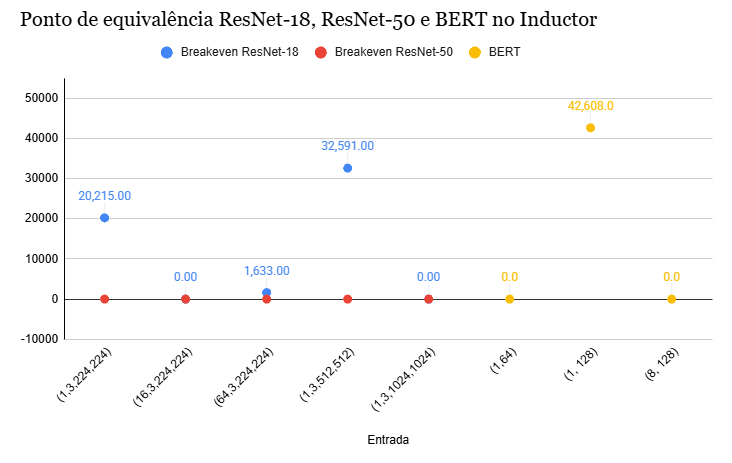
\includegraphics[width=0.9\linewidth]{images/equivalencia.png}
    \caption{Equivalence point (number of executions from which it is worth compiling with the fold pass) on the TorchInductor backend.}
    \label{fig:foldeq}
\end{figure}

This number is important because it is the break-even point between the cost of an optimization and the benefit it yields at execution. In ML systems, operator fusion is expensive: if a model is executed only a limited number of times, this cost may not be offset by the reduction in per-execution latency, and may even outweigh it. Making this threshold explicit is therefore useful whenever a system must decide, at deployment time, whether a given fusion or \emph{fold} pass is worth applying for the expected number of executions.

We performed the analysis of the fusion pass in isolation, but the proposed benchmark can be extended to other passes and other models.

\subsection{Proposed Benchmark}

We developed a \textit{benchmark} in which the user chooses the \textbf{model input} (\(N{\times}C{\times}H{\times}W\)) and the system runs, for each compiler, the standardized measurement of \textbf{compilation time} and \textbf{execution time per inference} for that input. At the end, the \textit{benchmark} reports (i) \emph{which compiler provides the best gain} for the number of executions of interest, and (ii) the \textbf{ranges of executions} in which \emph{each} compiler excels.

To ensure fairness in the comparison, \textbf{all compilers were configured equivalently}: the same architecture (ResNet-18/50), the same precision, the same device, the same layout when applicable (e.g., \emph{channels-last}/NHWC), \tcode{eval()} enabled, identical \emph{warmup} windows and number of iterations, plus congruent execution parameters (e.g., autotuning enabled when available). The orchestrator unifies metric collection and JSON serialization, ensuring reproducibility.

We model the total cost of each \emph{backend} \(b\) as \(T_b(n)=a_b\,n + b_b\), where \(a_b\) is the \textbf{average time per inference} and \(b_b\) is the \textbf{compilation time}. By constructing the \textbf{lower envelope} of these lines, we obtain the \textbf{crossover points} and, consequently, the \textbf{dominance ranges} of each compiler.

\paragraph{Report (\texttt{JSON}) and quick reading.}
The \textit{benchmark} generates a \texttt{JSON} file with: \textbf{meta} (experiment context), \textbf{raw} (measurements per \emph{backend}: \tcode{compile\_ms}, \tcode{exec\_ms}, \tcode{ttfb\_ms}), and \textbf{recommendation} (the \(T_b(n)\) model, crossover points, and dominance segments). The \tcode{best\_at\_runs\_exec} field directly indicates the best \emph{backend} for the given \(n\).

\begin{figure}[h]
    \centering
    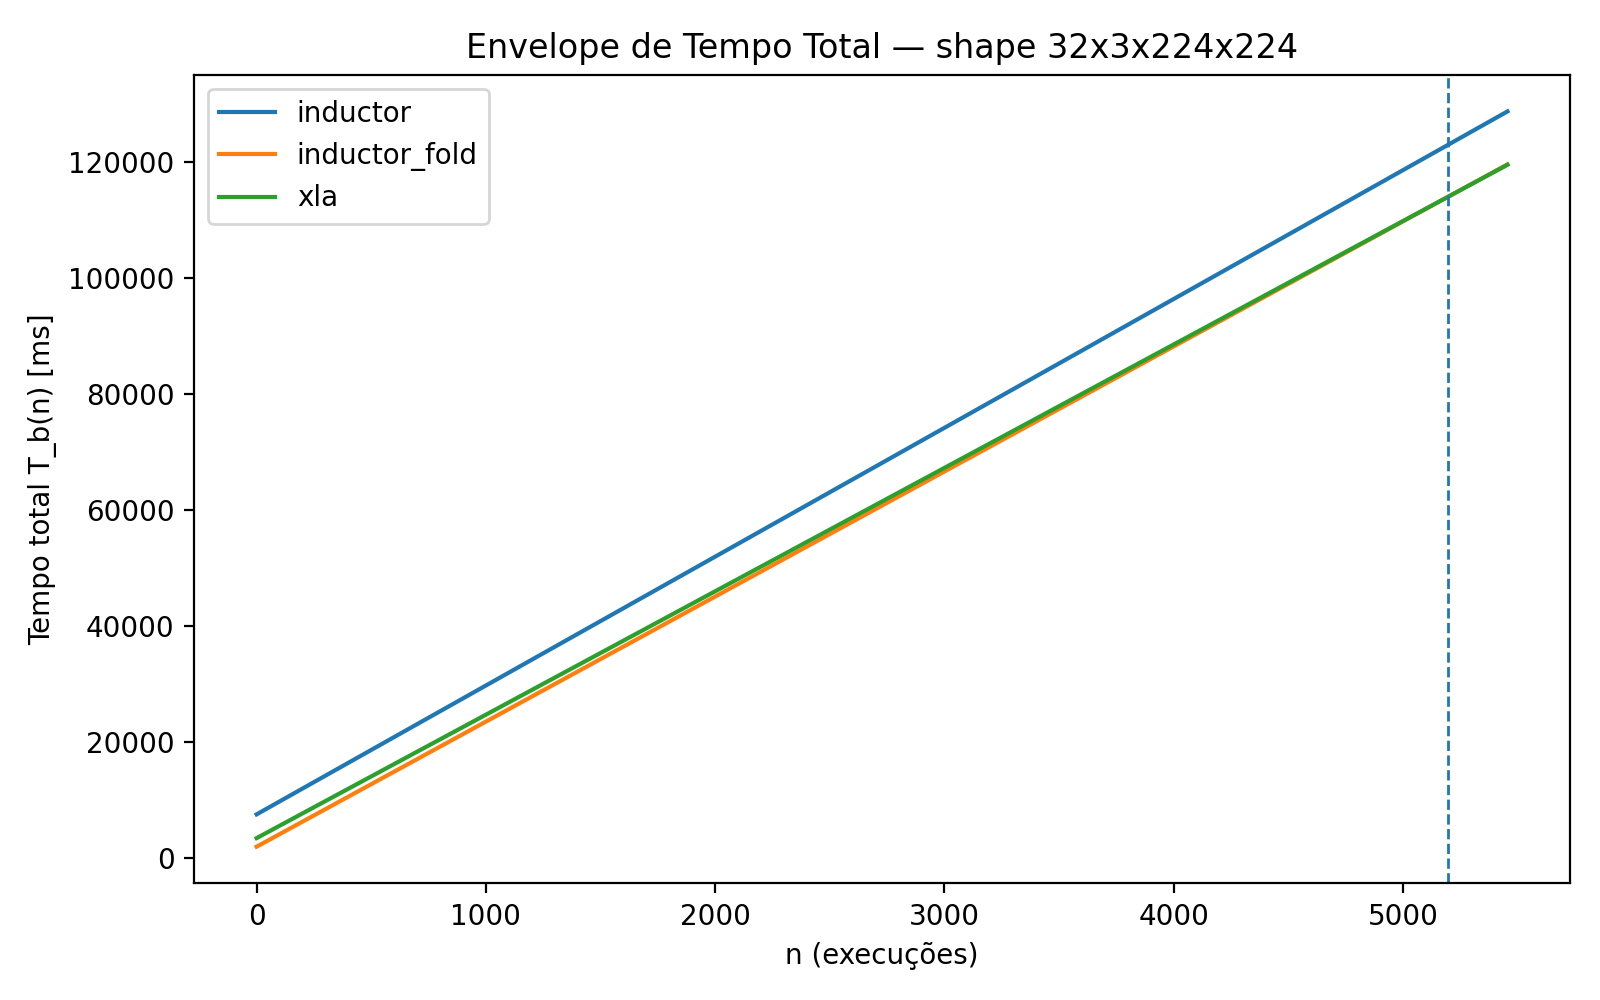
\includegraphics[width=0.9\linewidth]{images/envelope_exemplo.png}
    \caption{Example benchmark plot: lines \(T_b(n)=a_b n + b_b\) per \emph{backend}, with the lower envelope (dominance regions) and crossover points. In this example, \tcode{inductor\_fold} was best up to execution 5{,}197; from there on, XLA dominated.}
    \label{fig:envelope_exemplo}
\end{figure}

\paragraph{How to read Figure~\ref{fig:envelope_exemplo}.}
The \(y\)-axis starts at \tcode{compile\_ms} (intercept) and the slope is \tcode{exec\_ms}; the lower envelope highlights the winner in each range of \(n\); the intersections correspond to the crossover points (dashed vertical lines). If there are no intersections, the JSON comes with an empty \tcode{breakpoints} field and a single \tcode{segment}.

\section{Related Work}
\label{sec:related}

Operator fusion can be seen as the computation-graph analogue of classical \emph{peephole optimization}. Fraser's machine-independent peephole optimizer characterized valid local rewrites over a sequence of machine instructions by describing each instruction's effect as a Register Transfer List, replacing a window of instructions by a single equivalent one whenever such a description existed \cite{fraser1979peephole}. Operator fusion plays the same role one level up: where peephole optimization rewrites a window of three-address-code instructions into an equivalent instruction, fusion rewrites a window of computation-graph operators into an equivalent operator that preserves the observable semantics. In this sense, fusion is to the operators of a computational graph what peephole optimization is to instructions in a three-address-code representation. Among graph-level approaches, \emph{Optimus} minimizes memory accesses over the computation DAG through an offline dynamic-programming algorithm and an online buffer-budget variant \cite{cai2022optimus}. A practical limitation of such optimal-search formulations, however, is convergence: under a fixed time budget they often fail to reach the optimal fusion plan, and \citet{canesche2025xnnc} report that exhaustive search methods of this kind fail to converge on almost every large benchmark in their evaluation, which motivates the faster, heuristic strategies adopted by production compilers such as XLA, TVM, and TorchInductor.

\section{Conclusion}

This work presented a unified protocol for evaluating machine learning compilers (TorchInductor, XLA, and TVM), controlling \emph{inputs}, warmup, and the number of iterations, and introduced a decision criterion based on the \emph{lower envelope} of the total times \(T_b(n)=a_b n + b_b\), where \(a_b\) captures execution latency and \(b_b\) the compilation cost. The comparative analysis showed that differences in the handling of \emph{fusion} and of epilogues in libraries such as \tcode{cuDNN} explain much of the observed variation: XLA tends to benefit when it can delegate sequences such as \tcode{Conv+BatchNorm+ReLU} to a single \emph{custom call}, whereas TorchInductor, on the current \emph{inference} path, pays an overhead for \emph{codegen} and additional launches when emitting \tcode{BN+ReLU} as a separate kernel (via Triton). We also observed that each backend's dominance depends on the \(n\) regime: in situations with few executions, choices with cheaper compilation win; as \(n\) dominates, strategies with a higher degree of kernel fusion prevail.

\paragraph{Limitations.}
Despite the methodological care, there is still room to broaden the statistical robustness (e.g., reporting confidence intervals for all scenarios) and to diversify the environment (other GPUs/CPUs and \tcode{driver}/\tcode{cuDNN} versions). In addition, aspects of the CFG export may affect the fusion of non-canonical kernels in some backends.

Another limitation lies in the linearity assumption of the model \(T_b(n)=a_b n + b_b\) itself: by assuming that the per-batch cost is approximately constant and that all of the fixed cost is paid in the first batch, the model abstracts away cache effects, \emph{autotuning} strategies, and possible recompilations triggered by dynamic \emph{shapes}, which may make the effective behavior closer to a piecewise model than to a single line. In practice, the coefficients \(a_b\) and \(b_b\) should be read as summary statistics of the range of \(n\) that was measured, and not as exact predictions for any usage regime. Future work can refine this dimension by reporting goodness-of-fit metrics (for example, the regression's \(R^2\)) and by investigating nonlinear or \emph{piecewise} models in scenarios with greater temporal variability.

Beyond the comparison between backends, this work also evaluated \emph{fold} transformations in the \textbf{TorchInductor} graph, aiming to reduce the compilation cost without changing the model's semantics. In convolutional architectures (ResNet-18/50), folding \tcode{BatchNorm} into \tcode{Conv} reparameterizes the convolution's weights and biases and removes the explicit \tcode{BatchNorm} from the graph in \emph{eval} mode. This does not turn the \tcode{Conv+BatchNorm+ReLU} sequence into a single kernel---unlike XLA, which often delegates the whole chain to a single \emph{custom call}---but it reduces the volume of \emph{codegen}, since reparameterizing the \tcode{Conv} is much cheaper than generating a separate Triton kernel for \tcode{BN+ReLU}.

In attention-based models, such as BERT, we apply an analogous \emph{fold} on the \tcode{LayerNorm+Linear} combination: the affine part of \tcode{LayerNorm} ($\gamma$, $\beta$) is absorbed into the weights and biases of the subsequent \tcode{Linear}, so that TorchInductor now compiles only a ``pure'' \tcode{LayerNorm}, responsible solely for normalization. This eliminates the need for a more complex \tcode{LayerNorm} kernel (normalization + affine part) and reduces the associated \emph{codegen}, similarly to the effect observed with \tcode{BatchNorm}.

A key observation of our experiments is that TorchInductor does not apply folding automatically on the inference path, yet by applying it manually we obtained consistent compilation-time reductions and, in several cases, execution-time speedups. Since the Inductor is already a heavily optimized backend, this points to a broader research direction: generalizing the fold transformation and implementing it as an automatic pass inside the Inductor. As a direct first step, we intend to enable the fusion of \tcode{Conv+BatchNorm+ReLU} on the \emph{inference} path of \textbf{TorchInductor}. The proposal consists of (i) folding \tcode{BN} into \tcode{Conv} in \tcode{eval()} mode by adjusting \((W', b')\); (ii) triggering the \tcode{ReLU} epilogue directly in \tcode{cuDNN} via \tcode{aten::cudnn\_convolution\_relu(...)} (as happens in XLA); and (iii) integrating a \emph{pattern-rewrite} (FX/\tcode{torch.\_inductor.pattern\_matcher}) that detects \tcode{Conv$\rightarrow$BN$\rightarrow$ReLU} and falls back safely when the epilogue is not available. The evaluation of this fusion will be incorporated into our existing \emph{benchmark}, adding the new point to the \(T_b(n)\) \emph{envelope}. We expect to reduce TTFB and latency through a smaller number of Triton kernels and launches, widening the ranges in which TorchInductor dominates---bringing it closer to the profile observed when XLA delegates epilogues to \tcode{cuDNN}.

\section*{Acknowledgments}
The authors used \textbf{ChatGPT (OpenAI, 2025)} as a support tool during the
preparation of this paper, restricted to the following purposes: refining the
writing and checking textual coherence; reviewing the algebraic derivations of
the kernel fusions in Appendix~\ref{app:fusions}; and assisting in writing and
debugging portions of the benchmark code used in the experiments. All technical,
methodological, and analytical content is the authors' own and was reviewed and
validated by the authors. This disclosure follows the SBLP generative-AI policy
and the corresponding ACM, IEEE, and Springer guidelines.


\appendix

\section{Derivation of the Analyzed Fusions}
\label{app:fusions}

This appendix lists the three kernel fusions that are the focus of our benchmark. Throughout, $\odot$ denotes the element-wise (Hadamard) product, with broadcasting along the channel dimension when the operands' shapes differ.

\subsection*{BatchNorm + ReLU}
A widely known fusion combines a batch normalization (\tcode{BatchNorm}) followed by a rectified linear unit (\tcode{ReLU}). Let $X\in\mathbb{R}^{N\times C\times H\times W}$ be the activation tensor (batch, channels, spatial dimensions); $\mu\in\mathbb{R}^{C}$ and $\sigma^2\in\mathbb{R}^{C}$ the per-channel estimated mean and variance; $\gamma,\beta\in\mathbb{R}^{C}$ the learnable scale and shift; and $\varepsilon\in\mathbb{R}_{>0}$ the numerical-stability constant. \tcode{BatchNorm} computes
\begin{align}
\text{(I)}\qquad Y = \frac{X-\mu}{\sqrt{\sigma^2+\varepsilon}}\odot\gamma + \beta .
\end{align}
The \tcode{ReLU} is then applied element-wise to the output:
\begin{align}
\text{(II)}\qquad Z = \max(0, Y).
\end{align}
Realizing these two operations requires two kernels, (I) and (II). However, both can be carried out in a single kernel:
\begin{align}
\text{(III)}\qquad y = \max\!\left(0,\ \gamma\cdot\frac{x-\mu}{\sqrt{\sigma^2+\varepsilon}}+\beta\right).
\end{align}
Modern deep-learning compilers nonetheless cannot fuse every \tcode{BatchNorm+ReLU} pair, for reasons of coercion, dynamic behavior, and structural constraints in the program CFG (Section~\ref{sec:background}).

\subsection*{Conv + BatchNorm + ReLU}
In computer vision, the \tcode{Conv--BatchNorm--ReLU} chain is a natural fusion candidate. At inference, \tcode{BatchNorm} is a fixed linear transformation and can be absorbed into the convolution's weights and bias $(\tilde{W},\tilde{b})$; the \tcode{ReLU}, being element-wise, enters as an epilogue of the same kernel. The compiler then (i) recomputes $(\tilde{W},\tilde{b})$ incorporating the BN and (ii) applies the \tcode{ReLU} at the end of the kernel, eliminating intermediate tensors and extra launches. The arithmetic cost of the convolution is unchanged; the gain comes from reduced data movement and kernel orchestration.

Formally, let $X\in\mathbb{R}^{N\times C_{in}\times H\times W}$ be the input and $W\in\mathbb{R}^{C_{out}\times C_{in}\times K_H\times K_W}$, $b\in\mathbb{R}^{C_{out}}$ the convolution parameters. The pre-activation output is
\begin{align}
\text{(IV)}\qquad U_{n,c,h,w} = \sum_{c'=1}^{C_{in}}\sum_{r,s} W_{c,c',r,s}\,X_{n,c',h+r,w+s} + b_c .
\end{align}
\tcode{BatchNorm} at inference, with parameters $\mu,\sigma^2,\gamma,\beta\in\mathbb{R}^{C_{out}}$ and $\varepsilon>0$, is
\begin{align}
\text{(V)}\qquad Y_{n,c,h,w} = \frac{U_{n,c,h,w}-\mu_c}{\sqrt{\sigma_c^2+\varepsilon}}\,\gamma_c + \beta_c .
\end{align}
The \tcode{ReLU} (II) is then applied element-wise. Rewriting $Y_{n,c,h,w}$ in the form of kernel~(III), we absorb the \tcode{BatchNorm} into the convolution parameters by defining
\begin{align}
\text{(VI)}\quad \tilde{W}_{c,c',r,s} = \frac{\gamma_c}{\sqrt{\sigma_c^2+\varepsilon}}\,W_{c,c',r,s},\qquad
\text{(VII)}\quad \tilde{b}_c = \frac{\gamma_c}{\sqrt{\sigma_c^2+\varepsilon}}\,(b_c-\mu_c) + \beta_c .
\end{align}
Substituting into $Y$ and applying the \tcode{ReLU}, we obtain the \tcode{Conv+BatchNorm+ReLU} fusion in a single kernel:
\begin{align}
\text{(VIII)}\qquad Z_{n,c,h,w} = \max\!\left(0,\ \sum_{c'=1}^{C_{in}}\sum_{r,s}\tilde{W}_{c,c',r,s}\,X_{n,c',h+r,w+s}+\tilde{b}_c\right).
\end{align}
The inner term is exactly of the form of kernel~(III), now with the convolution already reparameterized by $(\tilde{W},\tilde{b})$.

\subsection*{LayerNorm (affine part) + Linear}
Analogously to the \tcode{Conv--BatchNorm--ReLU} case, we can exploit the structure of \tcode{LayerNorm} (LN) in \tcode{LN--Linear} chains, common in Transformer models such as BERT. For a single activation vector $h\in\mathbb{R}^{d}$, decompose the inference-time LN into (i) normalization (centering and rescaling by the standard deviation) and (ii) the affine part (scaling by $\gamma$ and shifting by $\beta$). Let
\begin{align}
\text{(IX)}\qquad \hat{h} = \mathrm{Norm}(h)
\end{align}
be the purely normalizing part of the LN, i.e., the vector centered and normalized using the mean and variance of $h$. The full LN is
\begin{align}
\text{(X)}\qquad \tilde{h} = \gamma\odot\hat{h} + \beta,
\end{align}
where $\gamma,\beta\in\mathbb{R}^{d}$ are the learnable scale and shift parameters. Suppose a \tcode{Linear} layer with weights $W\in\mathbb{R}^{m\times d}$ and bias $b\in\mathbb{R}^{m}$ follows. Its output is
\begin{align}
\text{(XI)}\qquad y = W\tilde{h} + b = W\big(\gamma\odot\hat{h}+\beta\big)+b .
\end{align}
Expanding,
\begin{align}
\text{(XII)}\qquad y = \underbrace{W\,\mathrm{diag}(\gamma)}_{W'}\,\hat{h} + \underbrace{(W\beta + b)}_{b'} .
\end{align}
Defining
\begin{align}
\text{(XIII)}\qquad W' = W\,\mathrm{diag}(\gamma),\qquad b' = W\beta + b,
\end{align}
we rewrite the \tcode{LN + Linear} composition as
\begin{align}
\text{(XIV)}\qquad y = W'\,\mathrm{Norm}(h) + b' .
\end{align}
That is, the affine part of the \tcode{LayerNorm} $(\gamma,\beta)$ can be absorbed beforehand into the \tcode{Linear} parameters, leaving the LN as a purely normalizing operation (without affine). In implementation terms, this lets the compiler (i) treat the LN as a simpler normalization kernel (fewer \tcode{mul}/\tcode{add} operations and fewer parameter tensors) and (ii) keep the \tcode{Linear} as an unchanged GEMM kernel, only with reparameterized weights and bias $(W',b')$. As in the \tcode{Conv--BatchNorm--ReLU} case, the total arithmetic cost of the \tcode{Linear} does not change; the benefit comes from simplifying the normalization kernels and reducing codegen work, especially in models with multiple LNs per block/layer.

\bibliographystyle{ACM-Reference-Format}
\bibliography{ref}

\end{document}